\subsection{Spielablauf}
\begin{center}
	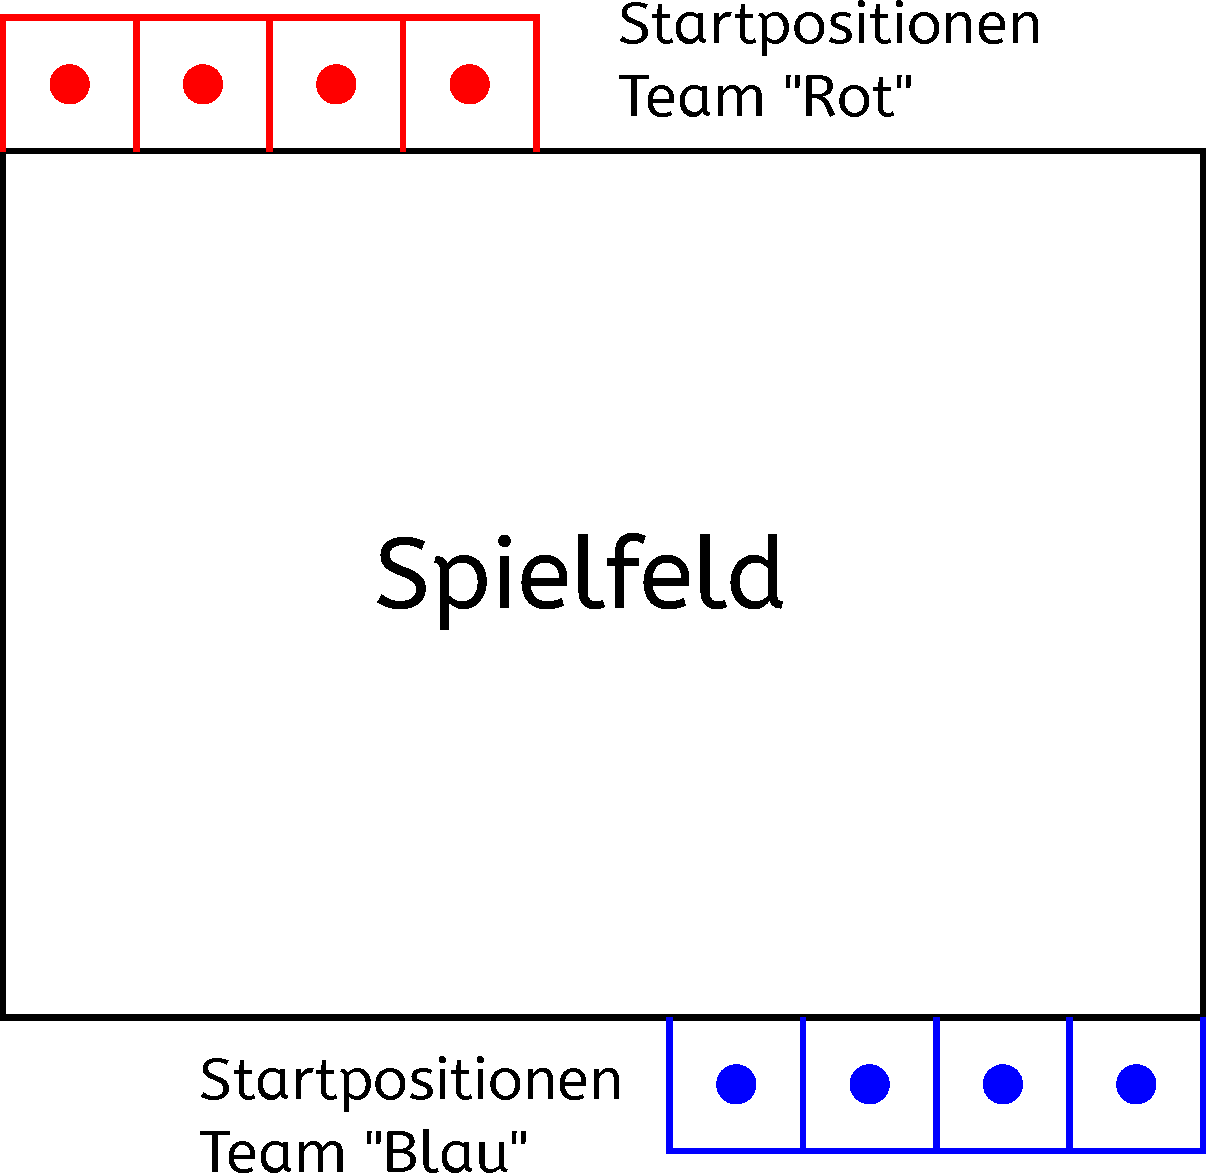
\includegraphics[width=0.5\textwidth]{Bilder/Spielfeld.pdf}
\end{center}
Es werden pro Gruppe 4 Roboter auf dem Spielfeld in extra Positionsfelder platziert.
Die Größe des Spielfeldes ist festgelegt.

\begin{enumerate}
	\item "'Start"' an den Server senden
	\item Warten auf Start vom Server
	\item Losfahren
	\item Geschwindigkeit: $\frac{3}{4}$ der vollen Geschwindigkeit
	\item Volle Geschwindigkeit ab einem Abstand x vom Gegner
	\item Meldung ob ein Roboter gefangen wurde, an den Server senden
	\item Server setzt den gefangenen Roboter auf neutral
	\item Gefangener Roboter fährt aus dem Spielfeld
	\item Spiel endet wenn alle Roboter einer Gruppe gefangen wurden bzw. nach 30 Minuten
\end{enumerate}